\clearpage\newpage
\subsection{Angle corrections} 
The $\theta$ angles of electrons and protons present  
a distorted $\phi$ dependence due mainly to misalignments
of the drift chambers. This error can be easily seen by looking at elastic events.
In particular one can calculate the predicted beam energy $E_{calc}$ using the angles of electron and proton with the formula

\begin{equation}
 E_{calc} = M_P-\Dfrac{M_P}{tan(\theta_e/2)\, tan\theta_P}
 \label{eqn:elastic_th}
\end{equation}
and look at the difference between $E_{calc}$ and the nominal beam energy $\Delta E = E_{nom}-E_{calc}$ 
as a function of $\phi$ (see \F{fig:energy_sec3}).

\begin{figure}[h]
 \begin{center}
  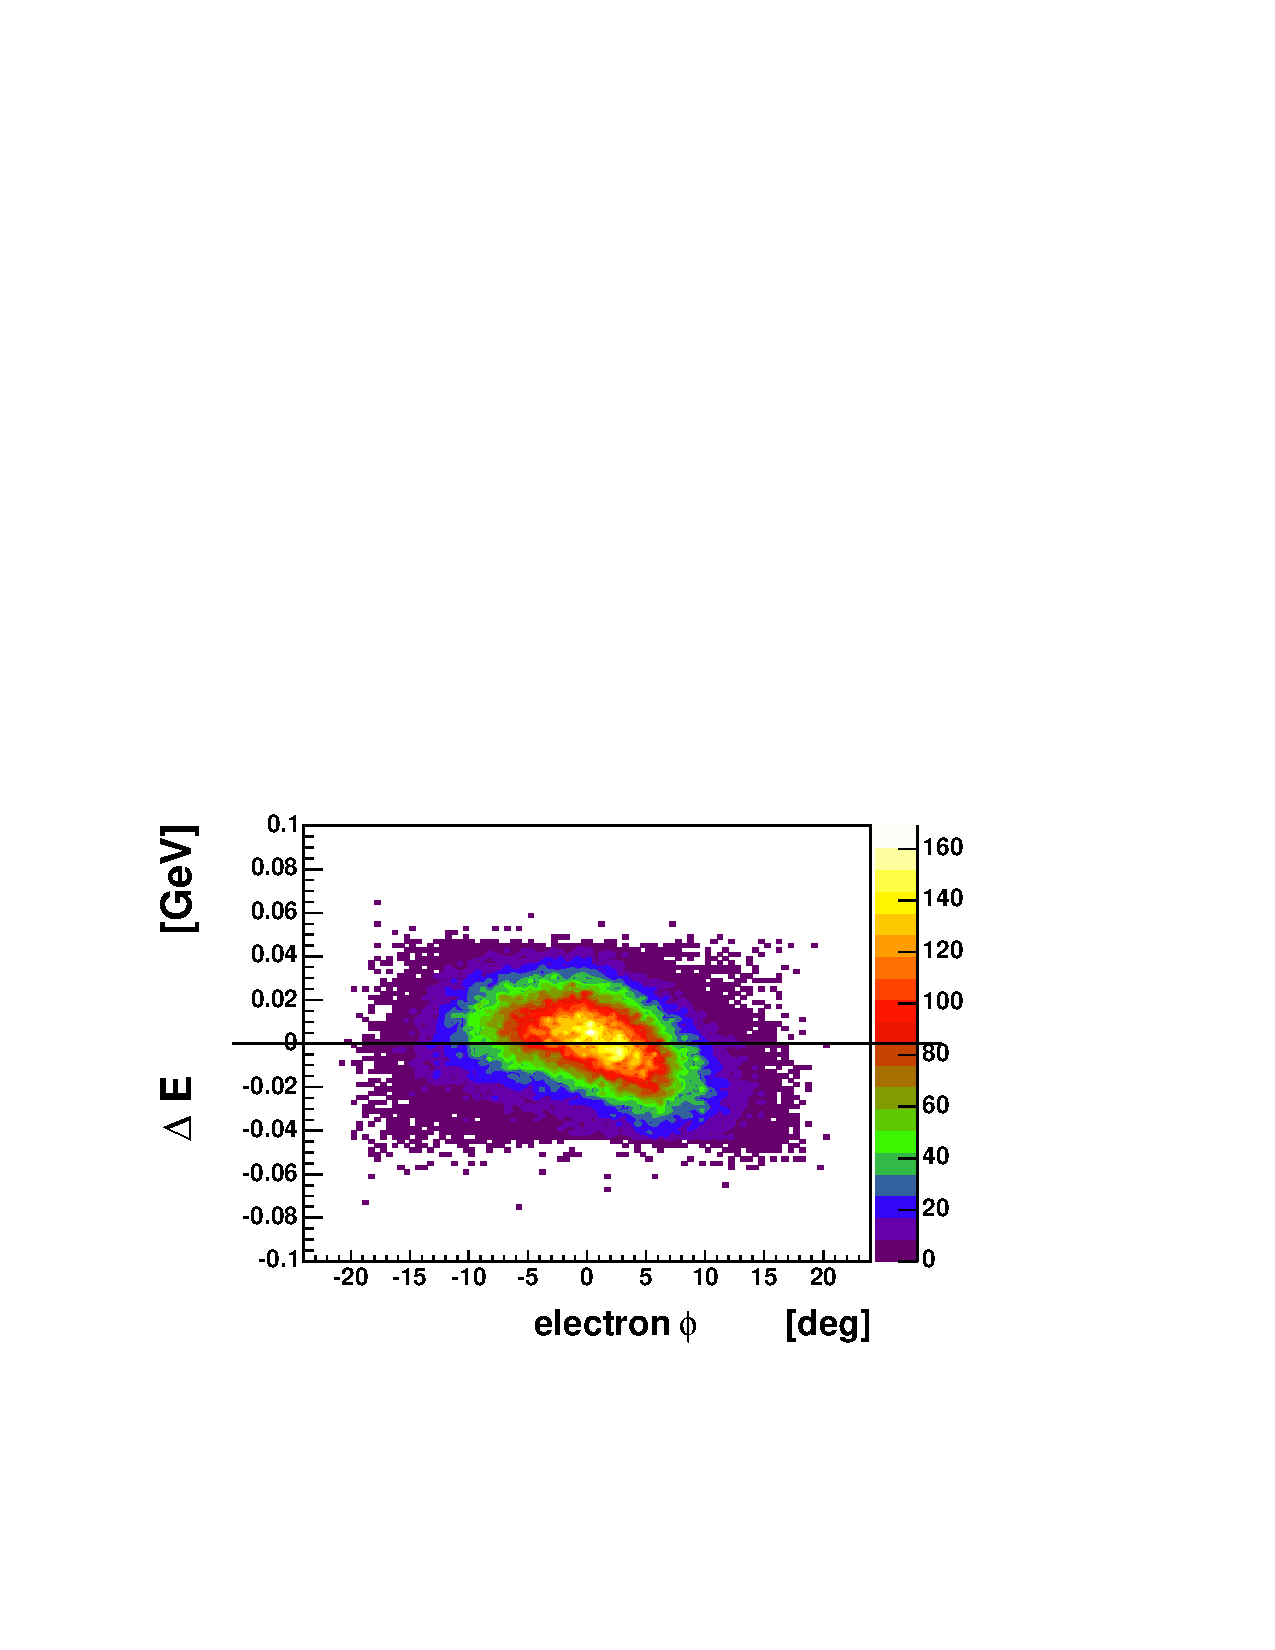
\includegraphics[width = 12cm, bb=40 130 500 440]{data_reduction/kine_corr/img/sector_3_energy}
  \caption[$\Delta E$ as a function of $\phi$ for electrons in sector3]
          { $\Delta E$ as a function of $\phi$ for electrons in sector3.
                     One can see distortions as big as $30$ MeV.}
 \label{fig:energy_sec3}
 \end{center}
\end{figure}
It turns out that the distortion is small, averaged around $0.4$ mrad ($0.02$ degrees) and 
peaking at $1$ mrad ($0.06$ degrees). However the momentum correction is based on the angle measurement.
Furthermore, the boost in the $\Delta^+(1232)$ c.m. system amplifies small deviations,
so the angles measurement have to be as precise as possible.

One can use (\ref{eqn:elastic_th}) to calculate a correction.
For example, one
can assume that the electron angle reconstruction is correct and calculate a correction
for the proton. Or vice versa.

In the present  work, it was assumed that the angle distortion comes from a DC misalignment,
and therefore gives similar effect on all particles. Under this assumption, all particles
have (the same) systematic error on their angle measurement,

In order to calculate the correction, the theoretical correlation (\ref{eqn:elastic_th}) between the lab angles
of the electron and proton is used. Such correlation is shown in \F{fig:elastic_theory}.
\begin{figure}[h]
 \begin{center}
 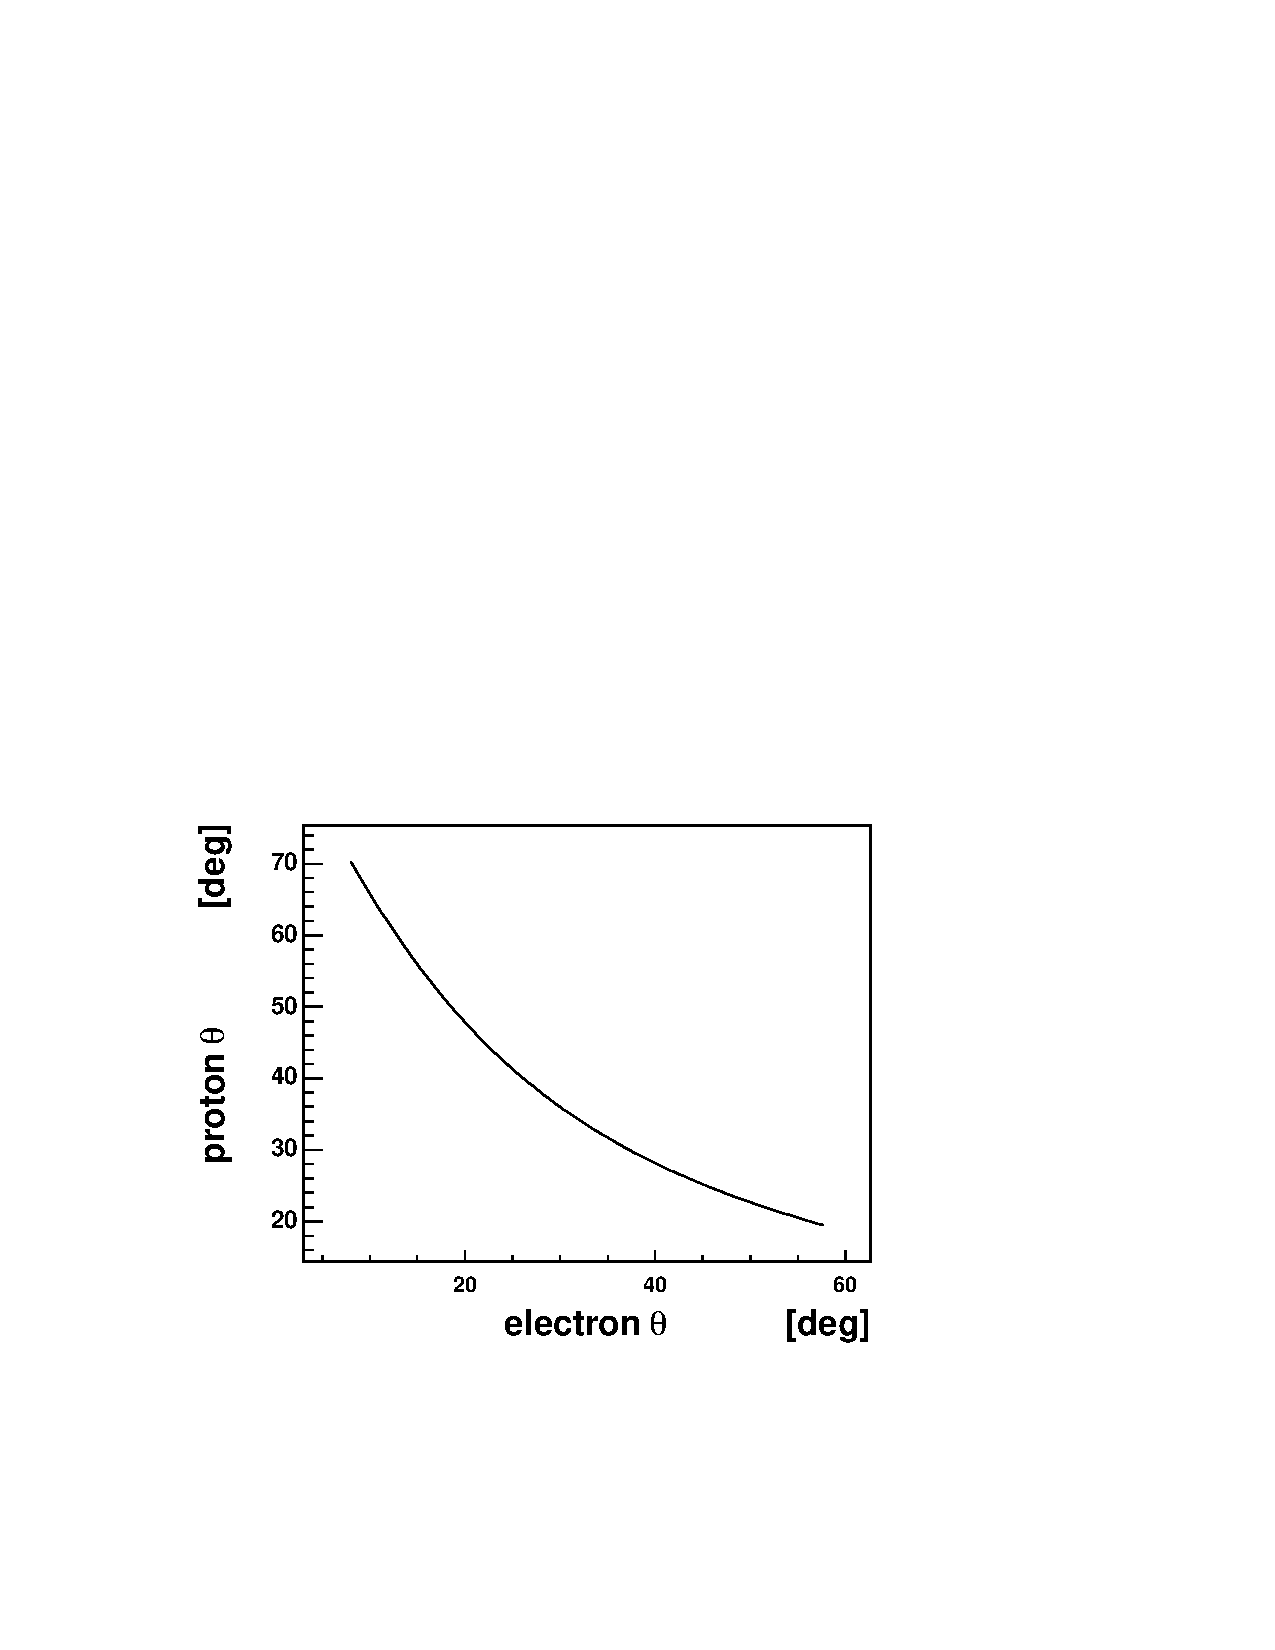
\includegraphics[width = 12cm, bb=60 120 500 420]{data_reduction/kine_corr/img/elastic_theory} 
  \caption[The constraint of elastic scattering]
          { The constraint of elastic scattering: proton $\theta$ versus electron $\theta$ 
                for elastic scattering for a $5.754$ GeV beam energy. }
 \label{fig:elastic_theory}
 \end{center}
\end{figure}

During the experiment, the measured angle P deviates from this curve as indicate in 
\F{fig:closer} which is a zoom of \F{fig:elastic_theory}. 
To calculate the corrections $\Delta\theta_e$ and  $\Delta\theta_p$ the point {\bf C} of the curve closest to
{\bf P} is found with an algorithm that minimizes the radius of a circle with center in {\bf P} intersecting the curve.

The corrections $\Delta\theta_e$ and  $\Delta\theta_p$ for the electrons and protons 
found with this algorithm then combined together and plotted for 
different $\theta$ slices in \F{fig:correction}. Notice that, since the correction is the same for all particles,
at this point electron and proton lose their identities and
``$\theta$'' is $\theta_e$ or $\theta_p$. 

\clearpage
\begin{figure}[h]
 \begin{center}
 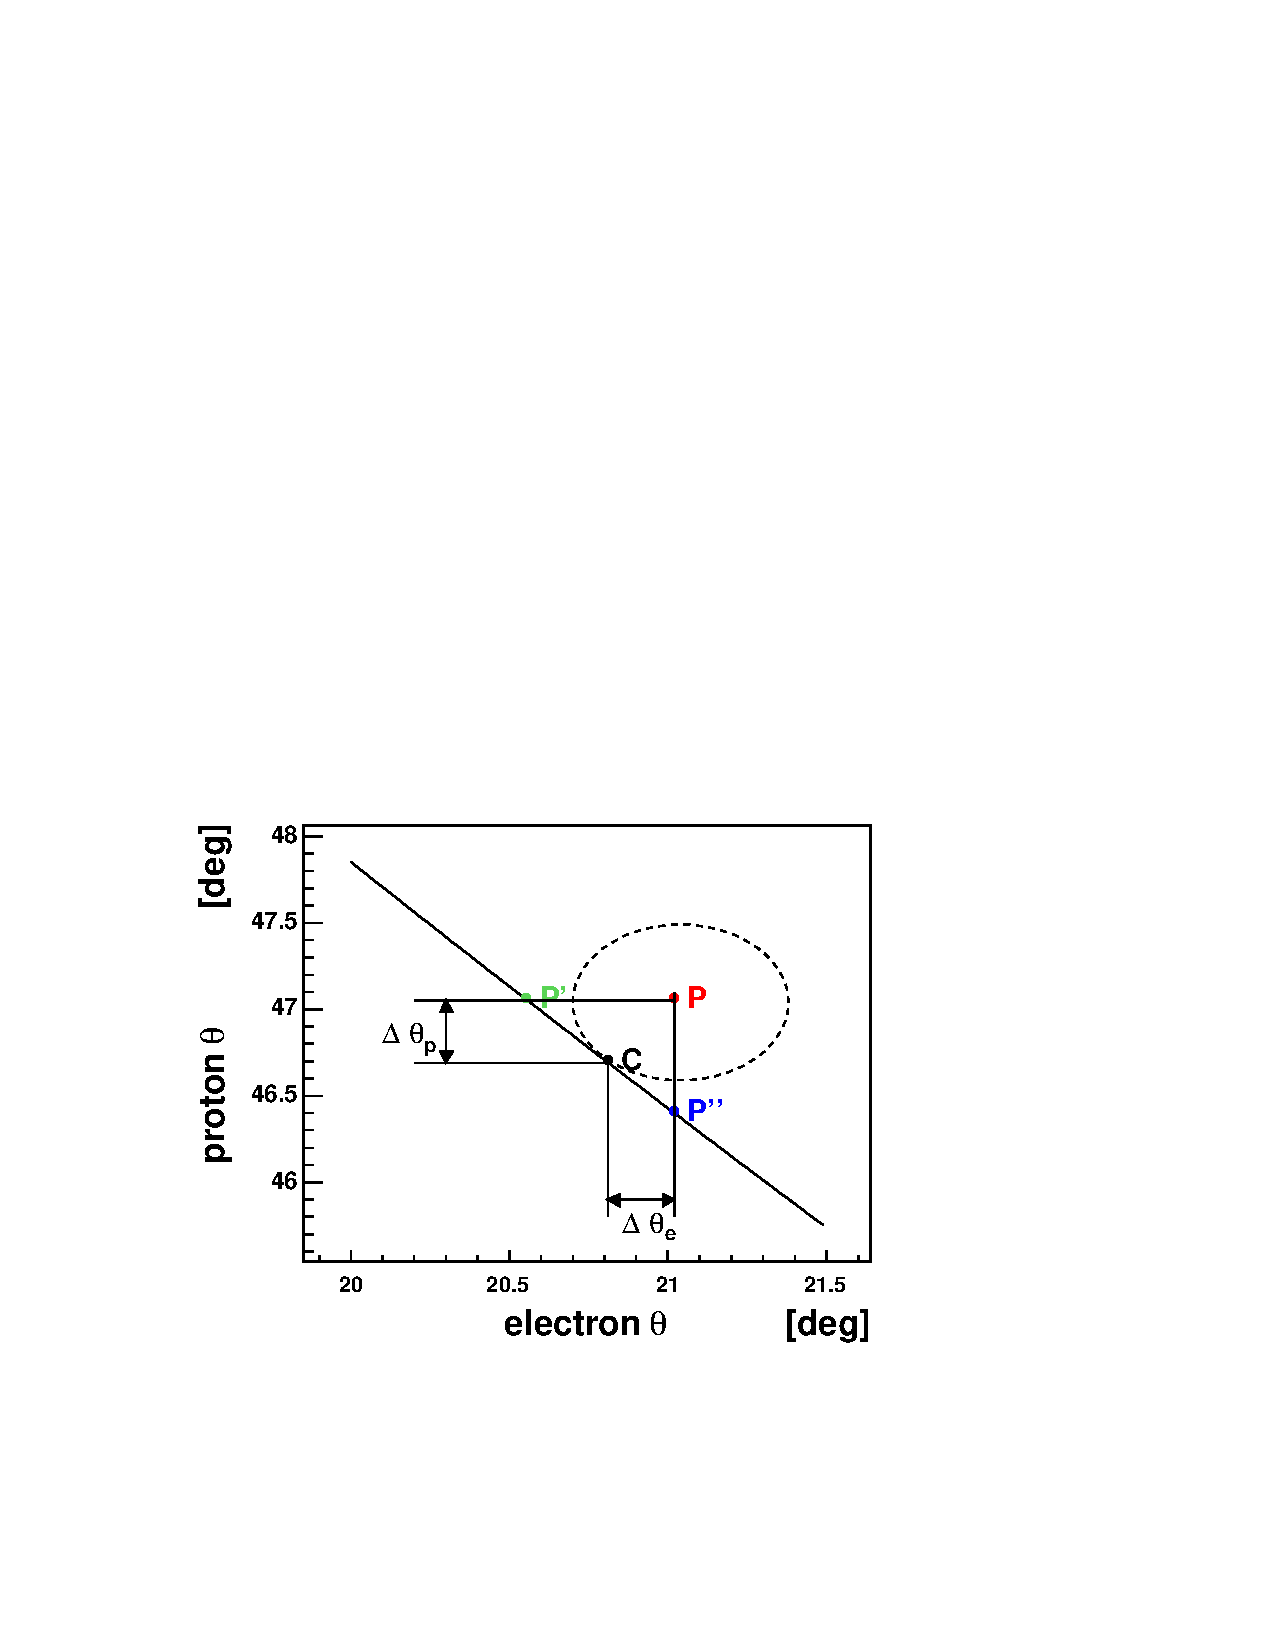
\includegraphics[width = 14cm, bb=60 120 440 520]{data_reduction/kine_corr/img/closer}
  \caption[The angle correction algorithm]
          { The angle correction algorithm. A measured angle of electron and protons (red point $P$) does not lie
                     in the theoretical curve. The circle with center
		     at $P$ intersecting the curve and with minimum radius is found. Its intersection with the curve
		     is the point $C$, the point of the curve closest to $P$. Notice that the x and y scales are different
		     so that the circle looks like an ellipse.}
 \label{fig:closer}
 \end{center}
\end{figure}

\begin{figure}
 \begin{center}
 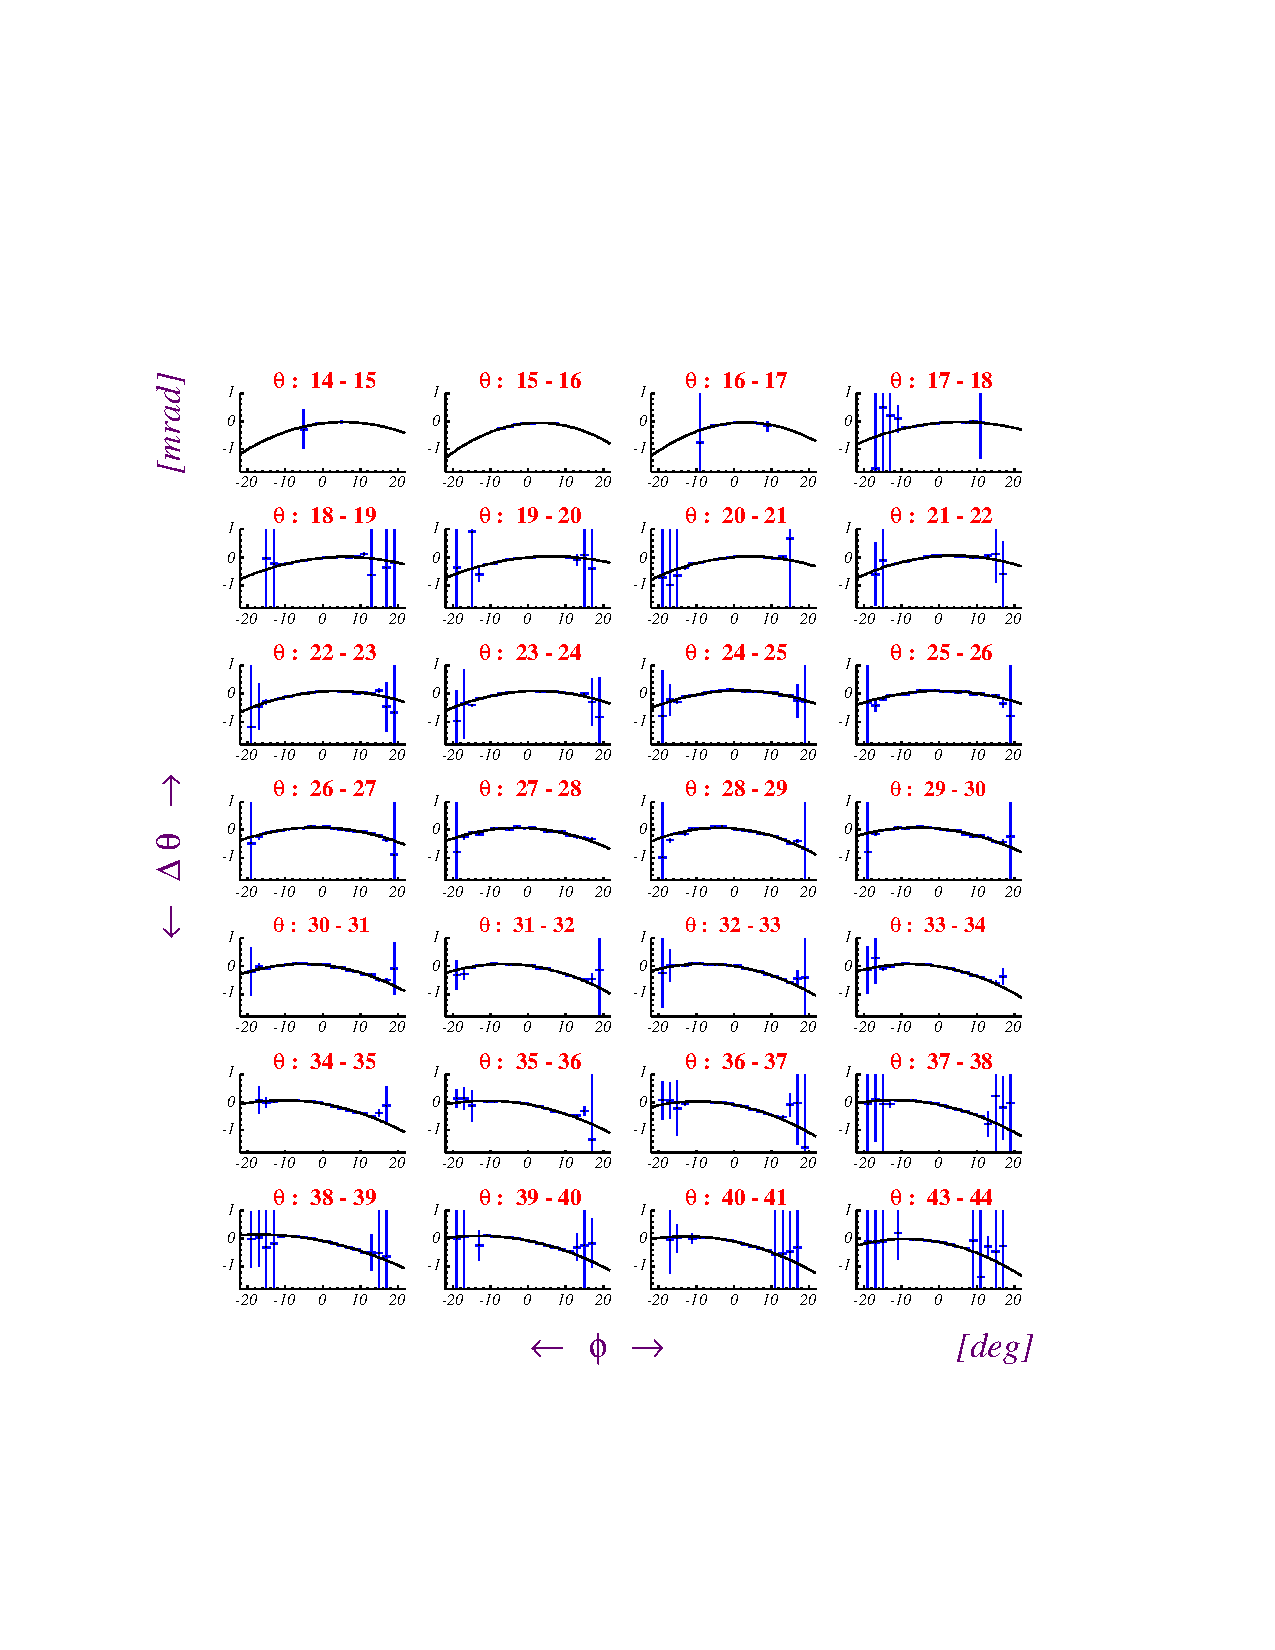
\includegraphics[width = 15cm, bb=60 120 540 650]{data_reduction/kine_corr/img/PHA}
  \caption[The combined angle correction for electron and proton for different $\theta$ slices]
          { The combined angle correction $\Delta\theta$ for electron and proton for 
                different $\theta$ slices. Each slice is fitted with a second order polynomial (black curve).}
 \label{fig:correction}
 \end{center}
\end{figure}
\cia
The correction is fitted with a second order polynomial, yielding three parameters for each $\theta$ slice considered:
$$
a = a(\theta)\, , \,\, 
b = b(\theta)\, , \,\,  
c = c(\theta)
$$
Each of the three parameters is then plotted as a function of $\theta$ in \F{fig:angle_pars_fit}.\\
When calculating the parameters for a given $\theta$ an interpolation is used, shown in the figure in red.
\begin{figure}[h]
 \begin{center}
  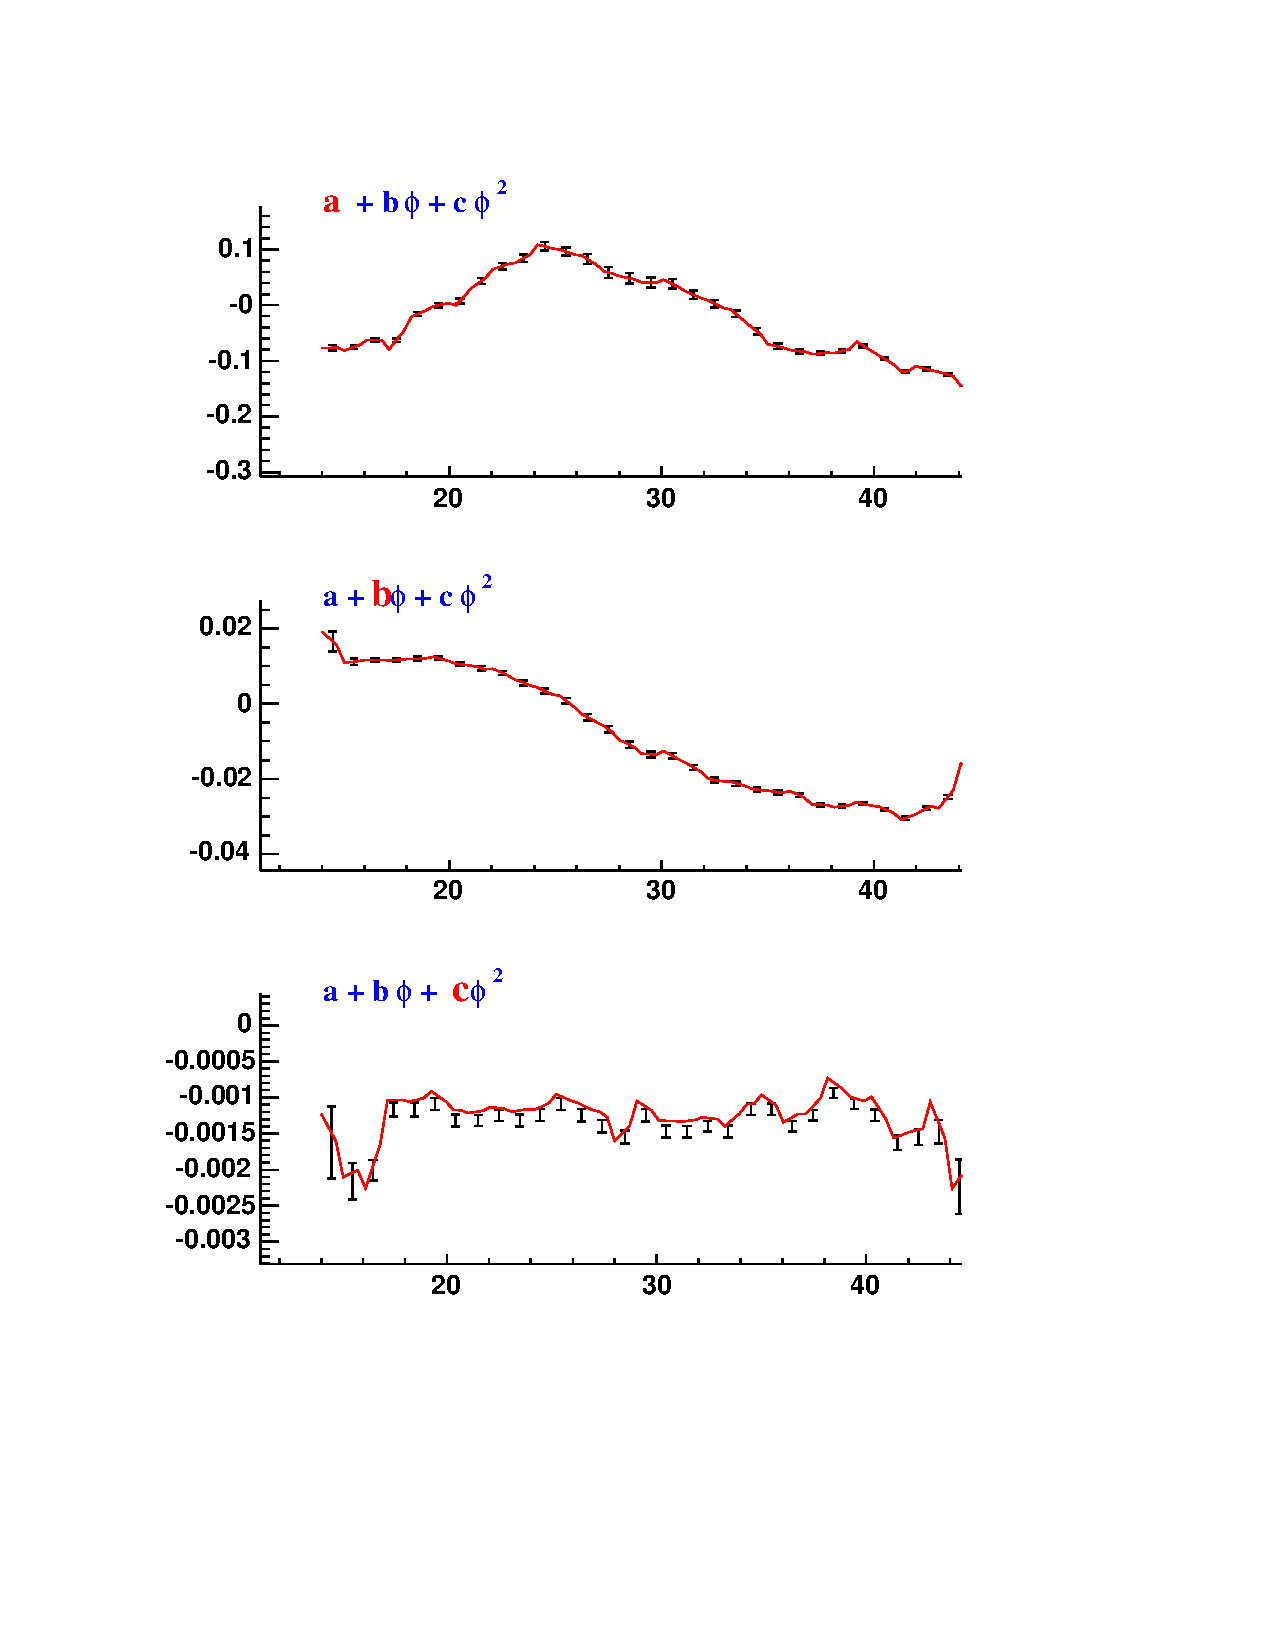
\includegraphics[width = 11cm, bb=0 100 550 720]{data_reduction/kine_corr/img/PART}
  \caption[Angle correction parameters as a function of $\theta$ for sector 1]
          { Angle correction parameters as a function of $\theta$ for sector 1. The red line is the linear
	             interpolation of the points.}
 \label{fig:angle_pars_fit}
 \end{center}
\end{figure}

\cia
The overall angles correction $\Delta\theta$ is \\
$$
\Delta\theta = a(\theta) + b(\theta)\,\phi + c(\theta)\,\phi^2
$$

To check to quality of the correction the $\Delta E$ distribution (like the one in \F{fig:energy_sec3}) is 
plotted against $\phi$ before and after the correction for each sector. \F{fig:angle_result} show 
the mean of the $\Delta E$ distribution.

\begin{figure}[h]
 \begin{center}
 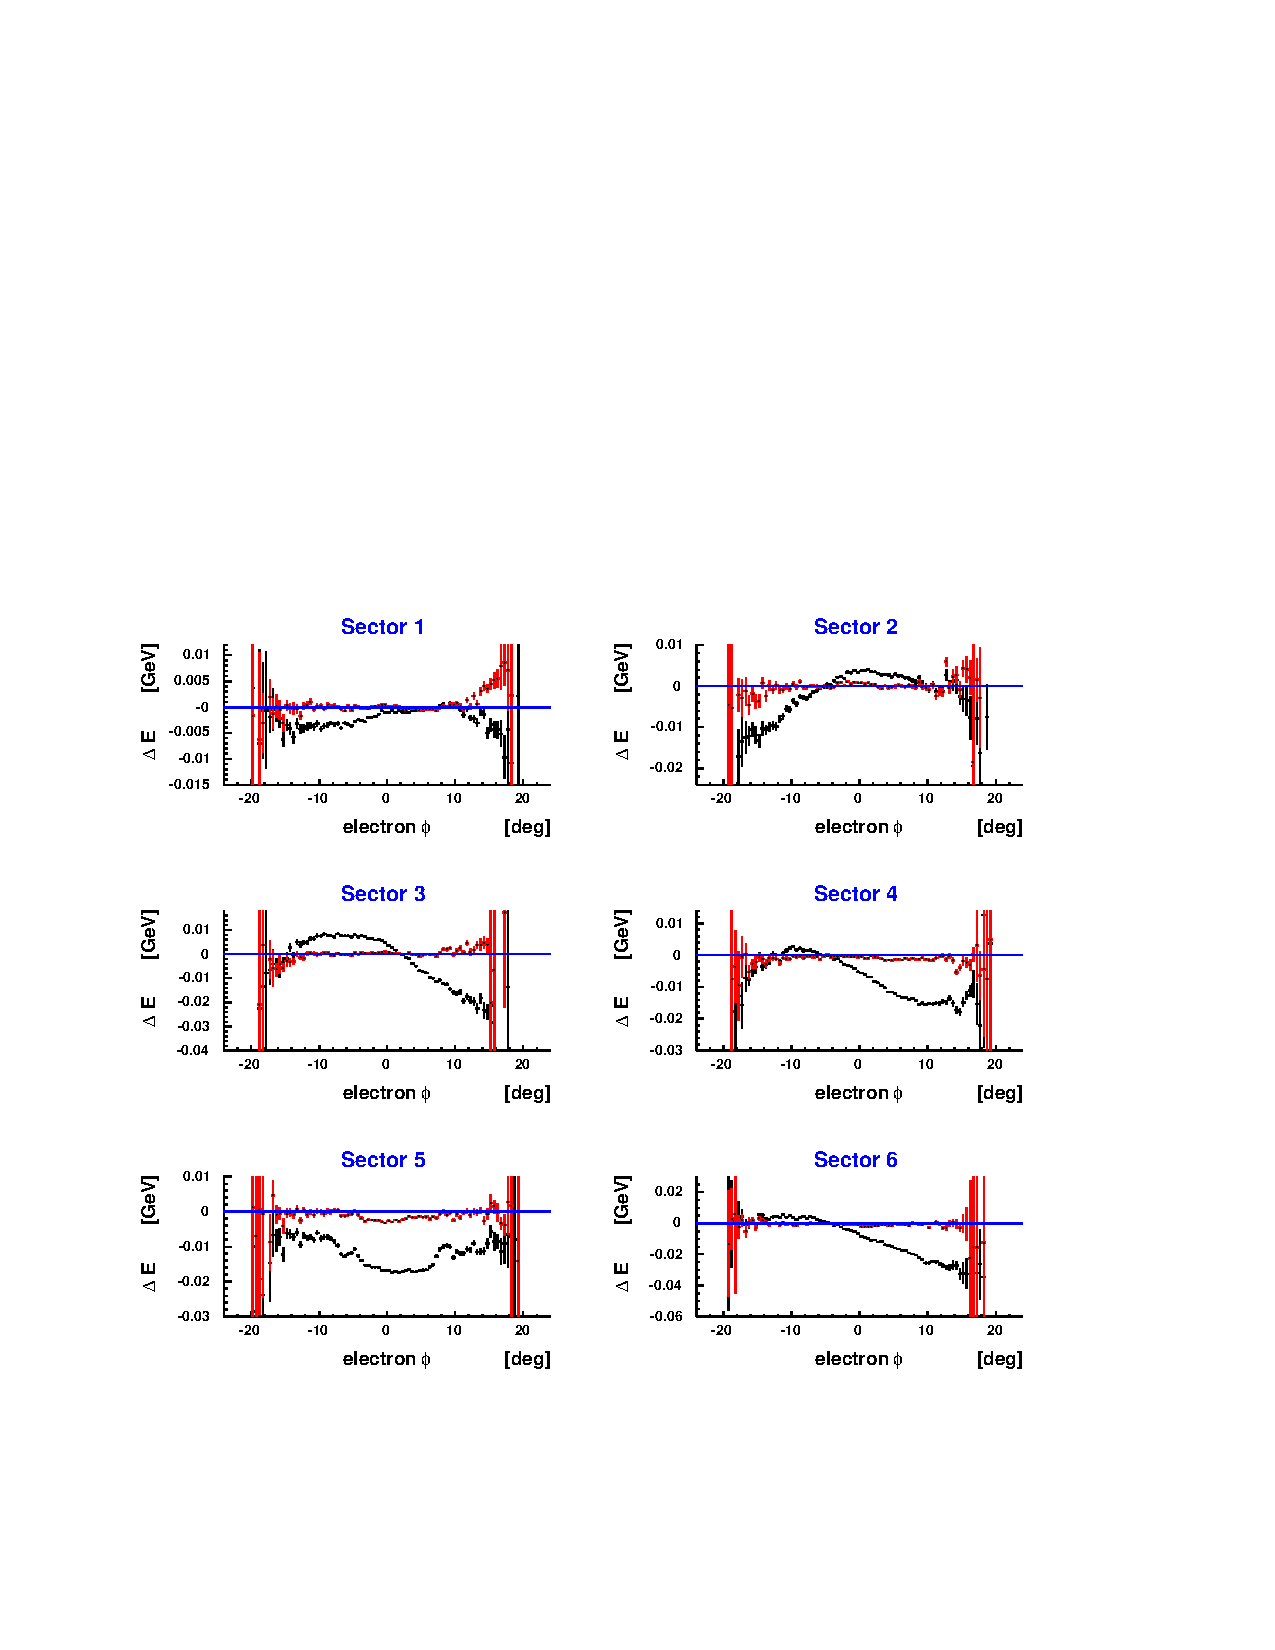
\includegraphics[width = 14cm, bb=30 120 550 570]{data_reduction/kine_corr/img/angle_result}
  \caption[$\Delta E$  as a function of $\phi$ for each sector]
          { $\Delta E$  as a function of $\phi$ for each sector. Black: before correction. Red: after correction. }
 \label{fig:angle_result}
 \end{center}
\end{figure}




\clearpage
\newpage


